\section{Experiments and Results}

There are an abundance of papers and studies that investigate the effect of imbalanced data and the diverse balancing algorithms in classification.
While researching for this project we saw many evaluation tables representing the performance of binary classifiers in a variety of circumstances.
We concluded that obtaining comprehensive results is beyond the scope of this team project, but we conducted experiments 
and we hope they can add something of value to the existing research, or at the very least, give the reader an overview of the overall challenges and tradeoffs involved.

There are some common truths established in previous research that we can state in advance.
For one, the number of available samples and the class imbalance ratio have a great effect on the success of any balancing method and classifier.
If there are only a handful of samples of the minority class available, because either the sample size is too low or the imbalance ratio to steep,
then no balancer or classifier will perform well.
One can also not hope for good performance if the number of features in which the class distributions have significant differences is too low, or
the sample clusters have too much overlap.

Our first experiment investigates this effect of class cluster distance in a simplified context of standard multivariate normal distributions.


\subsection{Cluster Distance Experiment}

When we conducted this experiment with the custom generator described in the previous section we came up with a function 
that generated the necessary parameter dictionaries for a standard multivariate distribution of i.i.d. components.
The idea was to have the mean of one cluster situated at the origin and the mean of the other at varying distance from it in the first orthant with all feature component
values being equal. We derived the corresponding for the latter mean like this:

Given a euclidian distance $d$ from the origin in $\mathbb{R}^n$, the coordinates of a vector $x \in \mathbb{R}^n$ with $x_1 = \dots = x_n$ are given by
\[
\begin{aligned}
	& \, d = \sqrt{ \sum_{j =1}^n x_j^2} = \sqrt{ n x_j^2} \\
	\Leftrightarrow& d^2 = n x_j^2 \\ 
	\Leftrightarrow& x_j = \frac{d}{\sqrt{n}} \\ 
\end{aligned}
\]

This formula for the coordinate components shows one of the faces of the phenomenon known as the "curse of dimensionality".
As the number of dimensions, $n$ in this case, increases the magnitude of the individual feature components decreases, bringing them closer to the origin.
So while the euclidian distances may be the same, the individual components of each cluster move closer together.
An algorithm that attempts to distinguish the clusters component-wise (as is necessary in the independent case we assume) will hence struggle severely to
distinguish the classes in higher dimensions. This is also what we observed in practice.

We ran the experiment with the FMLP pipeline using all combinations of unbalanced data, data balanced by \texttt{SMOTE}, \texttt{ADASYN}, \texttt{BorderlineSMOTE} and 
\texttt{SVMSMOTE} and the classifiers \texttt{LogisticRegression}, \texttt{DecisionTreeClassifier}, \texttt{Random Forest}, \texttt{XGboost} and \texttt{Lightgbm}.
These were used for all combinations of data with $10.000$ and $100.000$ samples, class ratios of $10\%$, $1\%$ and for $100.000$ also $0.1\%$ minority class,
and feature numbers $2,4,6,8$.
This produced a large table of some $4000$ entries that we intend to summarise here.

\begin{comment}
% for some reason this block does not work at all, while the others do
%\begin{tabular}{|r*{6}{|c}|}
\begin{tabular}{|*{6}{|c}|}
	\bfseries {cluster distance} & \bfseries accuracy & \bfseries precision & \bfseries  recall & \bfseries {F1 score} & \bfseries {ROC AUC Score} \\% specify table head
	%cluster distance & accuracy & precision & recall & F1 score &  ROC AUC Score % specify table head
	\csvreader[head to column names]{assets/tables/distance_mean_values.csv}{}{
	\csvcoli & \csvcolii & \csvcoliii & \csvcoliv & \csvcolv  & \csvcolvi %\thecsvrow &
	}% specify your coloumns here
	\\\hline
\end{tabular}
\end{comment}

We obtained the following table by grouping by the cluster distance and taking the mean across entries.
\begin{table}[H]
\centering
%\csvautotabular{assets/tables/distance_mean_values.csv}
\csvreader[
	tabular = *{6}{|c}|,
	table head = \hline \bfseries {cluster distance} & \bfseries accuracy & \bfseries precision & \bfseries  recall & \bfseries {F1-score} & \bfseries {ROC AUC Score}\\\hline, 
	late after line = \\\hline
	]{assets/tables/distance_mean_values.csv}{}{%
	\csvcoli & \csvcolii & \csvcoliii & \csvcoliv & \csvcolv  & \csvcolvi
}
\caption{Table aggregated by cluster distance}
\end{table}

What comes as no surprise is that the performance in every standard metric is on average better, the further the clusters are apart. 
Interestingly accuracy remains relatively high even for low distances while precision and F1-score decline dramatically when the clusters are close.
This demonstrates the "inadequacy of accuracy" (cite) as a measure of classifier performance in this context.

For sample sizes of $100.000$ and class ratio $0.1\%$ the balancing process failed at cluster distance $1$. 
At this point the clusters have some much overlap and the minority class is in comparison so underrepresented 
that attempting to find a minority class nearest neighbour to a minority class sample is often in vain.
Another interesting insight is that in general the balancing step takes significantly longer the lower the distance between the clusters.
At a distance of $4$ or $5$ FMLP completes the balancing step in seconds, while at a distance of $1.5$ or $1$ this step took up to half an hour to complete or failed entirely.

When we instead group and aggregate the performance metrics by the balancer used we obtain the following table:

\begin{table}[H]
\centering
%\csvautotabular{assets/tables/distance_mean_values.csv}
\csvreader[
	tabular = *{6}{|c}|,
	table head = \hline \bfseries {balancer} & \bfseries accuracy & \bfseries precision & \bfseries  recall & \bfseries {F1-score} & \bfseries {ROC AUC Score}\\\hline, 
	late after line = \\\hline
	]{assets/tables/dist_bal_mean_values.csv}{}{%
	\csvcoli & \csvcolii & \csvcoliii & \csvcoliv & \csvcolv  & \csvcolvi
}
\caption{Table aggregated by balancing method}
\end{table}

We can see that both recall and AUC values are on average significantly improved by balancing the data.
Precision however can be seen to decrease across balancing algorithms compared to training on unbalanced data.
Considering that recall is higher but precision is lower we can conclude that the overall rate of false positives increases when using a balancing algorithm.
This is most likely due to the often criticised (cite) tendency of balancing methods to lead to systematic over-prediction of minority class probabilities.\cite{harm_imbalance}
We will show this tendency more clearly in the section on calibration curves.

For completeness we also aggregated by classification method.

\begin{table}[H]
\centering
%\csvautotabular{assets/tables/distance_mean_values.csv}
\csvreader[
	tabular = *{6}{|c}|,
	table head = \hline \bfseries {classifier} & \bfseries accuracy & \bfseries precision & \bfseries  recall & \bfseries {F1-score} & \bfseries {ROC AUC Score}\\\hline, 
	late after line = \\\hline
	]{assets/tables/dist_clsf_mean_values.csv}{}{%
	\csvcoli & \csvcolii & \csvcoliii & \csvcoliv & \csvcolv  & \csvcolvi
}
\caption{Table aggregated by classification method}
\end{table}

The scores are fairly similar, but what seemed surprising to us was that a simple decision tree, which we mainly included for reference, 
performed only marginally worse than its corresponding ensemble method: random forest.


\subsection{Mode Experiment}

For this experiment we attempted to investigate how a situation, where one of the class distributions is bimodal, affects the outcome of the balancing and classification steps.
The dataset we generated for this has one million samples in $15$ dimensions and a class imbalance ratio of $0.5\%$. 
The majority class has two modes, one at $\mu_{0,1} = (-5)_{j=1}^{15}$ and one at $\mu_{0,2} = (5)_{j=1}^{15}$ with i.i.d. components 
and a variance of $\Sigma_{0,1} = 2 \mathbf{I}$ and $\Sigma_{0,2} = 0.7 \mathbf{I}$ respectively, where $\mathbf{I} \in \mathbb{R}^{15 \times 15}$ is the unit matrix.
The minority class is unimodal and has mean $\mu_{1} = (0)_{j=1}^{15}$ and covariances $\text{cov}(X_i^1, X_j^1) = 1$ for $i \neq j$ and $\text{cov}(X_i^1, X_i^1) = 2$.
Plotting $20.000$ of these samples in any two dimensions in a scatterplot gives us this picture:

\begin{figure}[H]
  	\centering
  	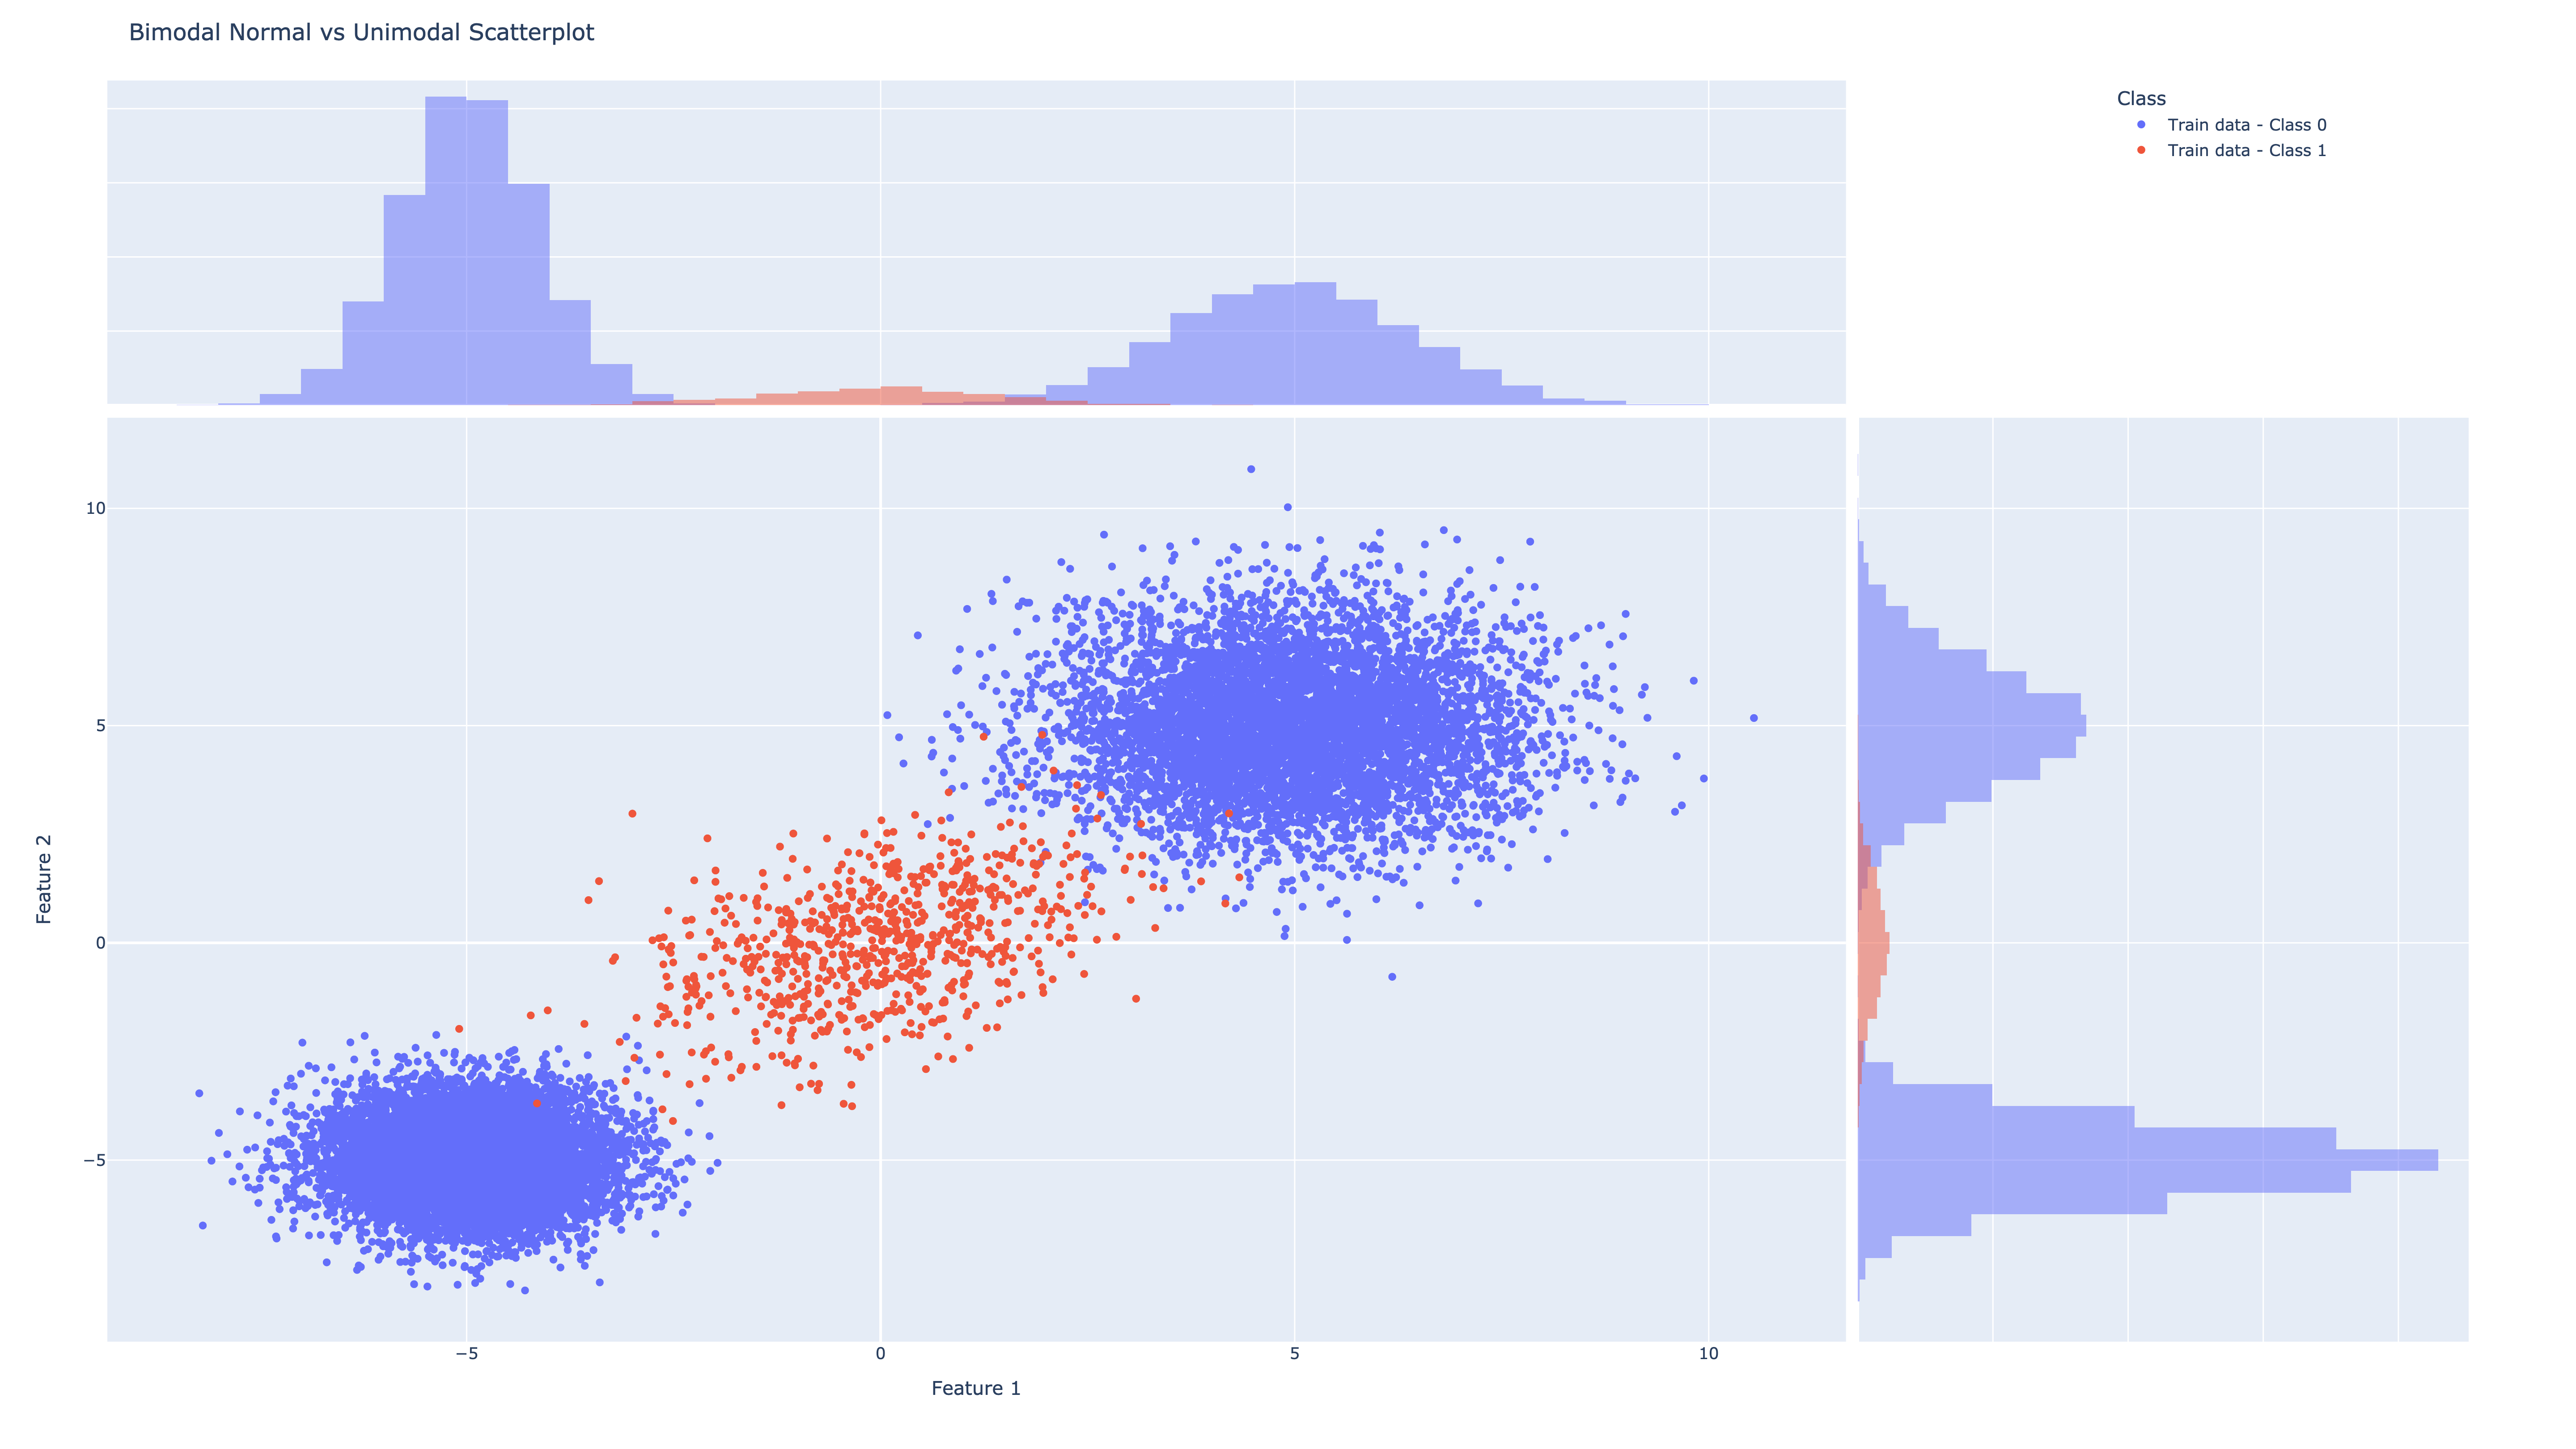
\includegraphics[width=\linewidth]{assets/data_vis/Bimodal_Maj_Unimodal_Min.png}
  	\captionof{figure}{Bimodal Majority vs Unimodal Minority Scatterplot}
  	\label{fig:Mode_Experiment}
\end{figure}

While it is relatively straightforward to determine the means and covariance matrices to have the distributions look as desired in two dimensions, 
it was not easy in $15$ dimensions. 
Enforcing adequate distances feature-wise, maintaining the desired structure and guaranteeing that the covariance matrix is actually symmetric and positive semi-definite,
is difficult if one wants the distributions to be non-trivial. 
Here we settled for a simple but non-trivial approach to keep the data understandable for the reader.
We again used the same balancers and classifiers as in the distance experiment. 
One notable occurrence during the execution of the pipeline was, that fitting \texttt{Random Forest}, typically a fast method, took an exceptionally long time,
namely more than all the other classifiers involved put together.  
This long fitting time might be due to the bimodal setup of the dataset: As a random forest algorithm randomly splits the dataset ahead of time, it could be that subsets 
are chosen that complicate finding splits that reduce entropy.

We hence decided to forego rand

















